\documentclass{beamer}
\usepackage[utf8]{inputenc}
\usepackage{pdfpages}
\usepackage{graphicx}
\usepackage{listings}
\usepackage{color}

\definecolor{mygreen}{rgb}{0,0.6,0}
\definecolor{mygray}{rgb}{0.5,0.5,0.5}
\definecolor{mymauve}{rgb}{0.58,0,0.82}

\lstset{ %
  backgroundcolor=\color{white},   % choose the background color
  basicstyle=\footnotesize,        % size of fonts used for the code
  breaklines=true,                 % automatic line breaking only at whitespace
  captionpos=b,                    % sets the caption-position to bottom
  commentstyle=\color{mygreen},    % comment style
  escapeinside={\%*}{*)},          % if you want to add LaTeX within your code
  keywordstyle=\color{blue},       % keyword style
  stringstyle=\color{mymauve},     % string literal style
  language=Java,
  basicstyle=\ttfamily
}

\lstset{literate=%
{Ö}{{\"O}}1
{Ä}{{\"A}}1
{Ü}{{\"U}}1
{ß}{{\ss}}2
{ü}{{\"u}}1
{ä}{{\"a}}1
{ö}{{\"o}}1
}

\usetheme{Berkeley}

\title{PK0}
\subtitle{Zusatzkurs für Programmieranfänger im WS 16/17}
\author{Marvin Gülzow}
\institute{Universität Konstanz}
\date{2016-10-26}

\begin{document}
\frame{\maketitle}

\begin{frame}
\frametitle{Inhalt}
\tableofcontents
\end{frame}

\section{Übersicht}
\begin{frame}{\secname}
Heute: 
\begin{enumerate}
\item Allgemeine Studientipps
\item Eclipse installieren
\item Erstes Programm zum Laufen bringen
\end{enumerate}
\end{frame}

\begin{frame}{\secname}
Später: 
\begin{enumerate}
\item Kontext: Wo läuft mein Programm?
\item Vorlagen zum Programmieren
\item Grundlegende Programmelemente
	\begin{itemize}
	\item Befehle
	\item Variablen
	\item Bedingungen
	\item Schleifen
	\end{itemize}
\item Fehlerquellen und Fehlersuche
\item Effiziente Verwendung von Editoren
\item Versionskontrolle
\item Programmierstil
\item Kollaboratives Programmieren
\end{enumerate}
\end{frame}

\begin{frame}
\frametitle{Kursziele}
\begin{itemize}
\item Zuerst: Starthilfe
\item Wiederholung von PK1
\item ``Denkweise'' des Programmierens vermitteln
\end{itemize}
\end{frame}

\section{Vorstellung}
\frame{\sectionpage}
{
\setbeamercolor{background canvas}{bg=}
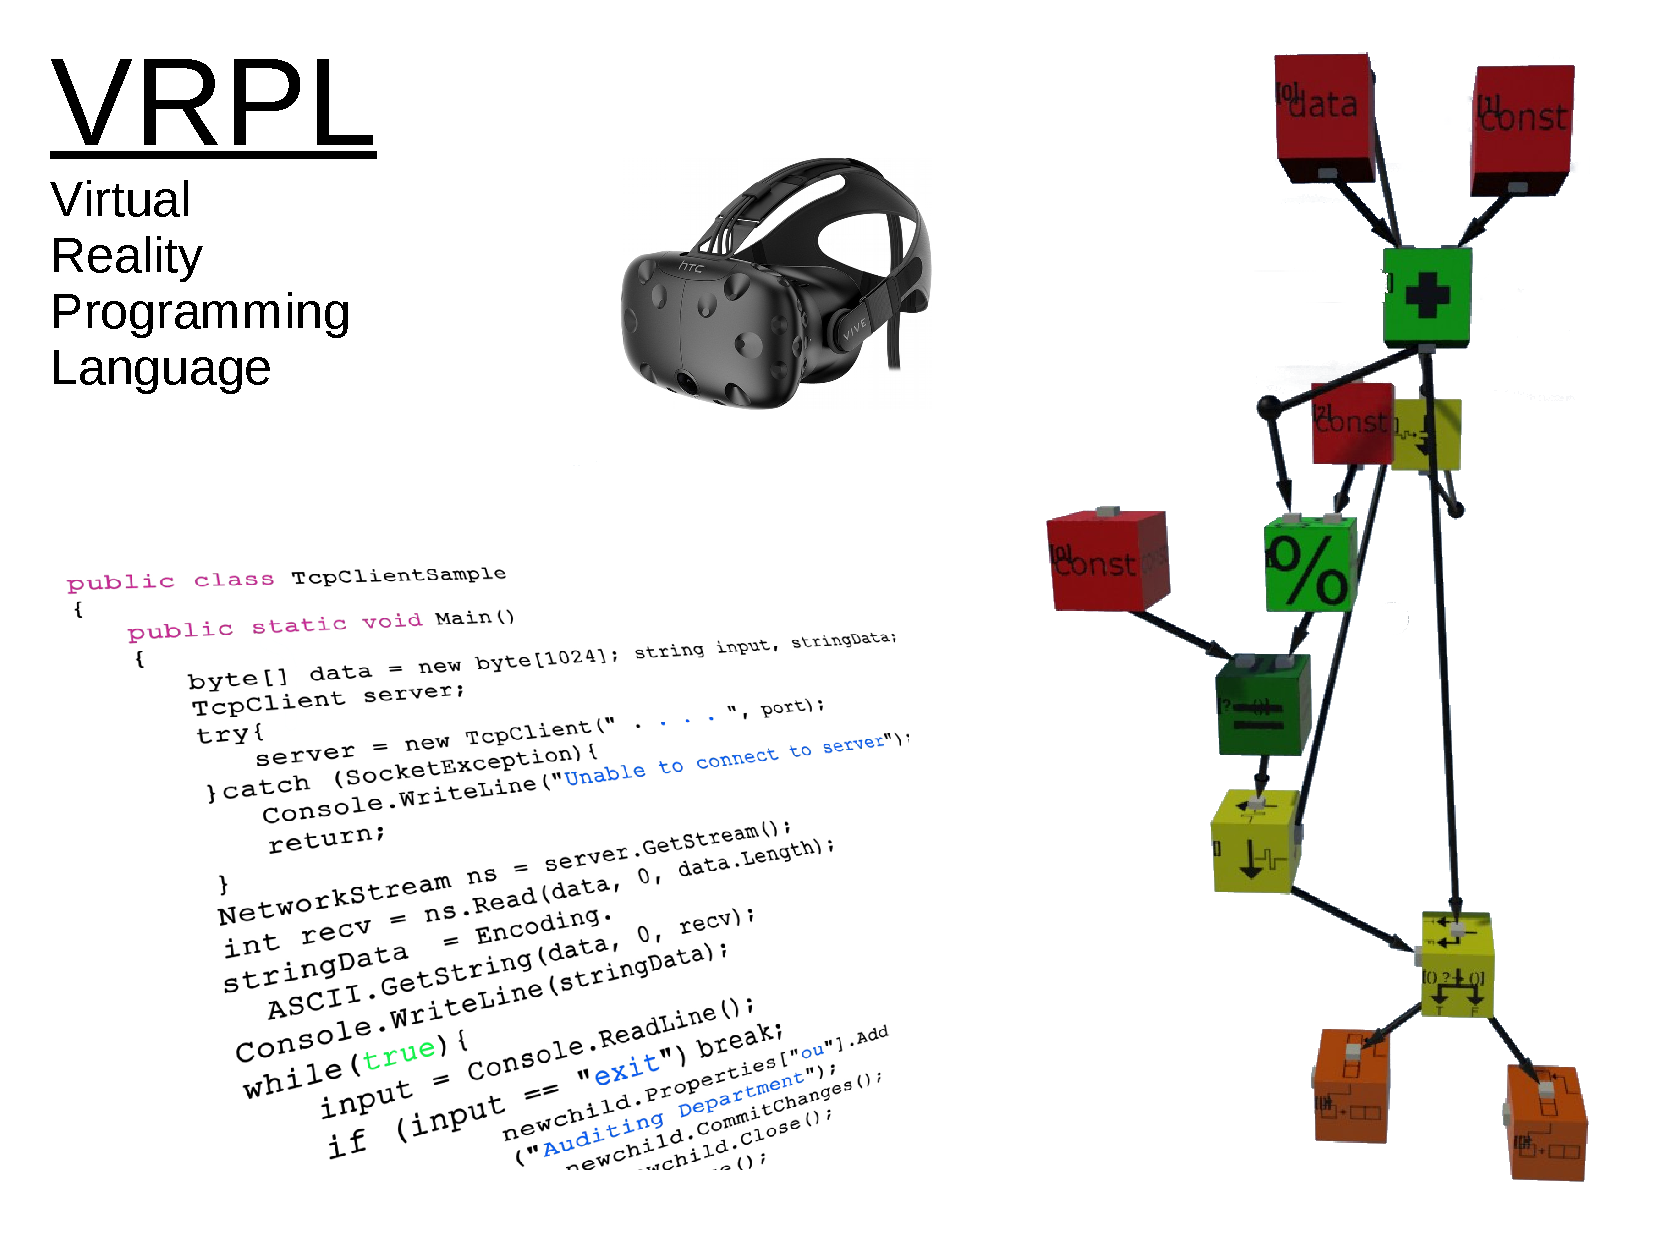
\includepdf[pages=1]{self.pdf}
\includepdf[pages=2]{self.pdf}
\includepdf[pages=3]{self.pdf}
}

\section{Studientipps}
\begin{frame}{In Vorlesungen gehen}
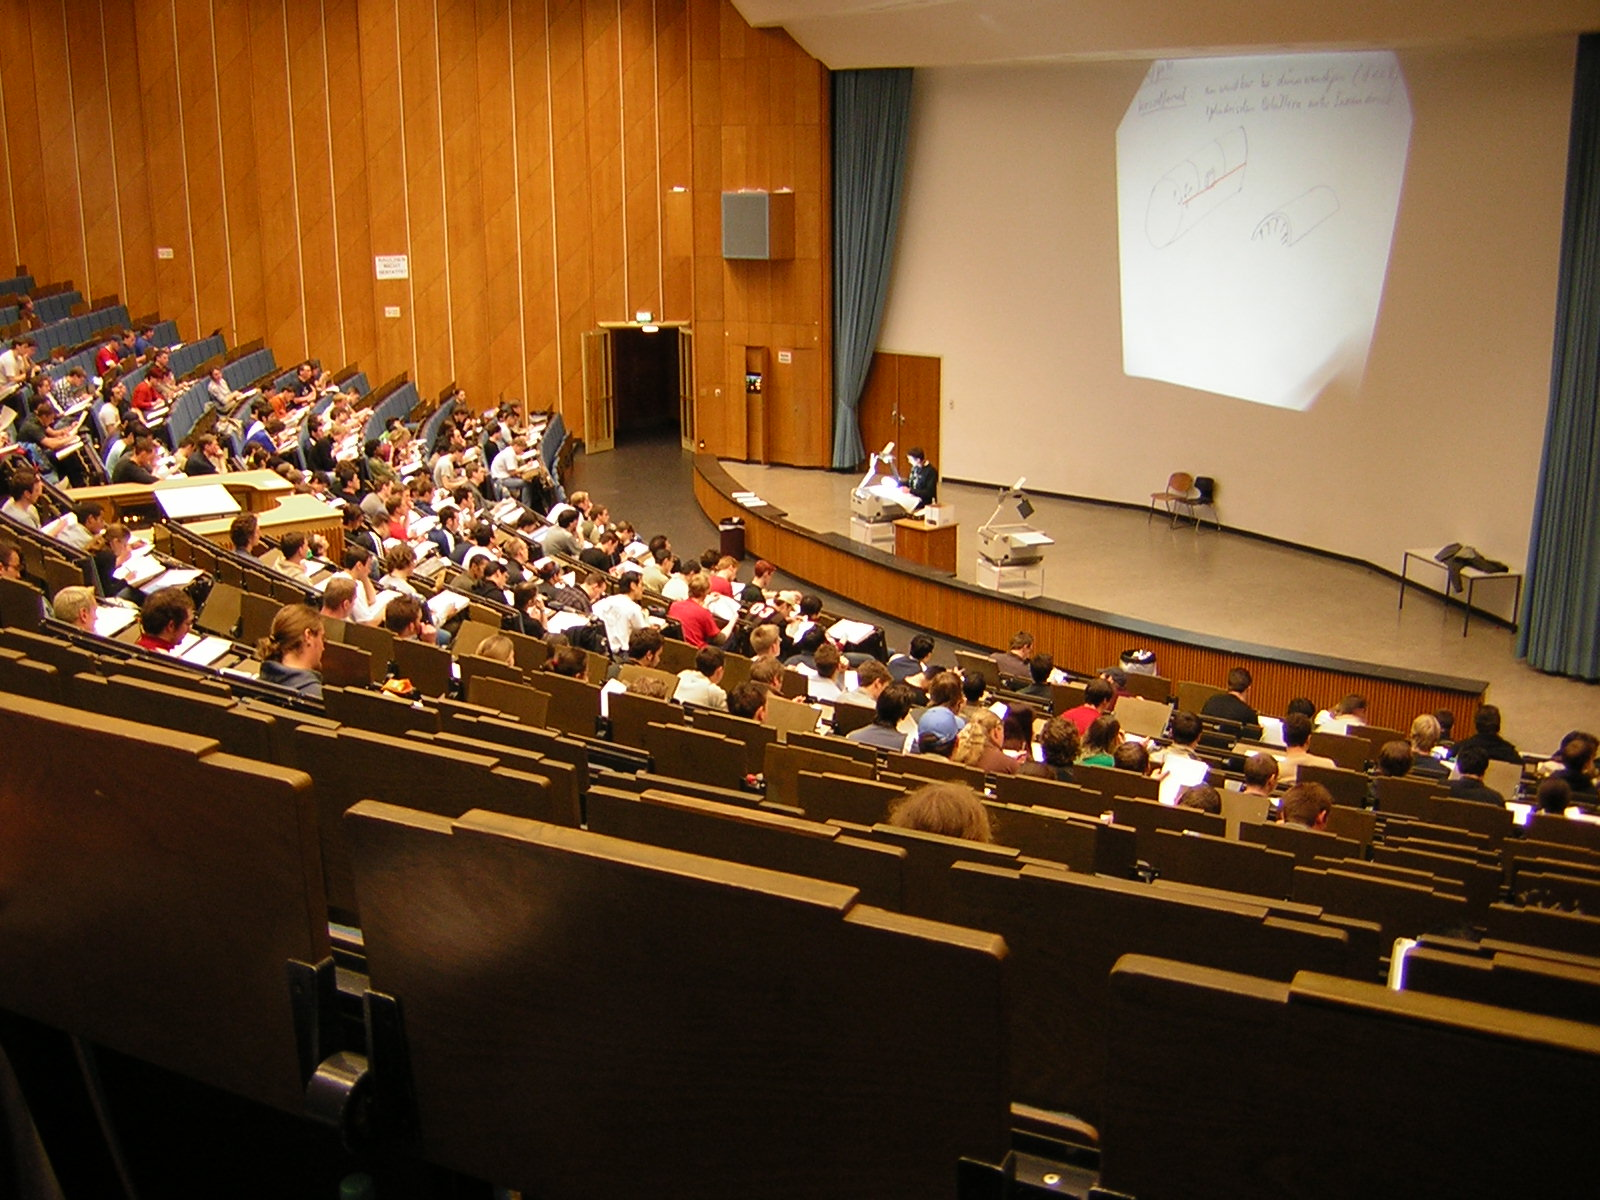
\includegraphics[width=\textwidth]{img/lecture.jpg}
\end{frame}

\begin{frame}{Vorlesung == Klausurvorbereitung}

\includegraphics[width=\textwidth]{img/nopass.jpg}
\end{frame}

\begin{frame}{Vorlesung == Klausurvorbereitung}
\begin{itemize}
\item Mein Jahrgang: 80\% ausgeschieden
\item Ablauf:
	\begin{itemize}
	\item Erstversuch
	\item Zweiversuch
	\item \textbf{Härtefallantrag}
	\item Verlust des Prüfungsanspruchs $\Rightarrow$ Exmatrikulation
	\end{itemize}
\item \textbf{Achtung:} Fachwechsel Inf $\rightarrow$ IE erst im dritten Semester möglich (Herrn Brunner für Genaueres fragen)
\end{itemize}
\end{frame}

\begin{frame}{Notebooks aus}
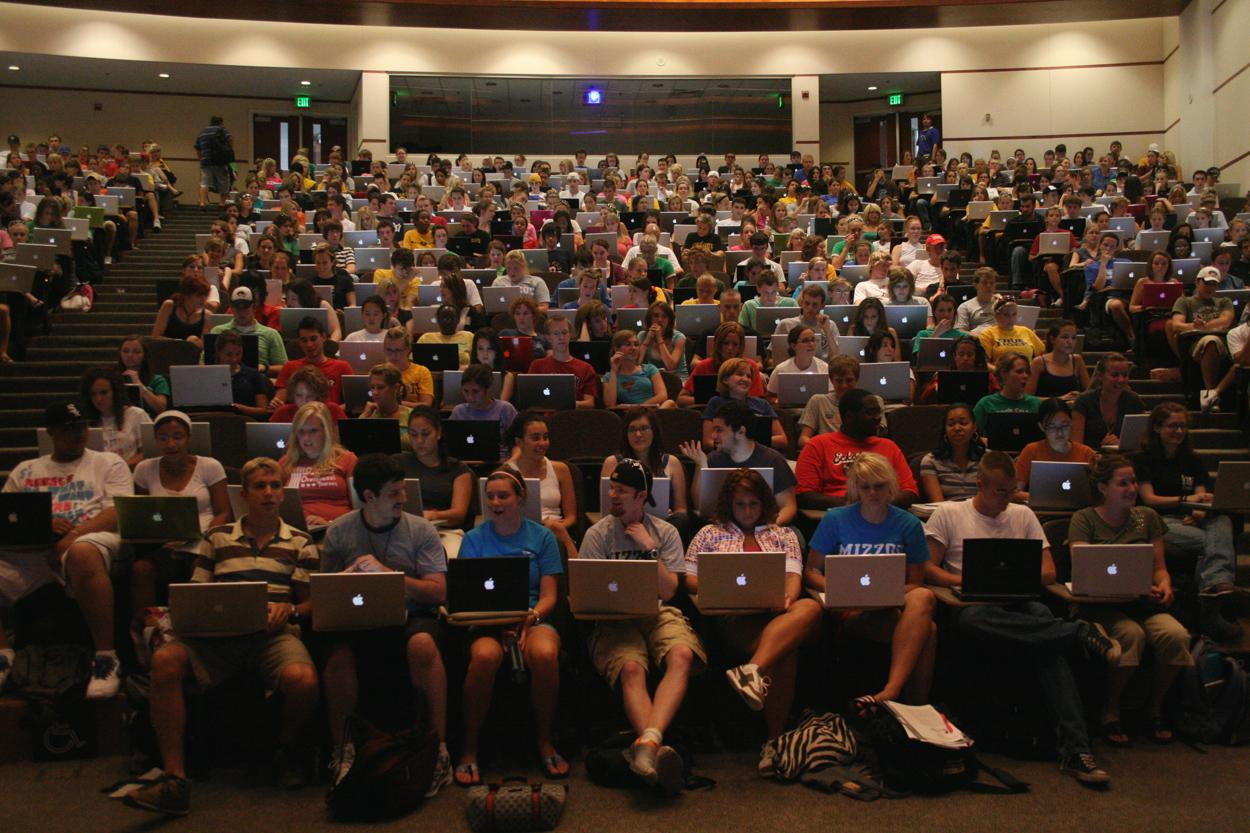
\includegraphics[width=\textwidth]{img/notebooks.jpg}
\end{frame}

\begin{frame}{Kooperation}
\centering
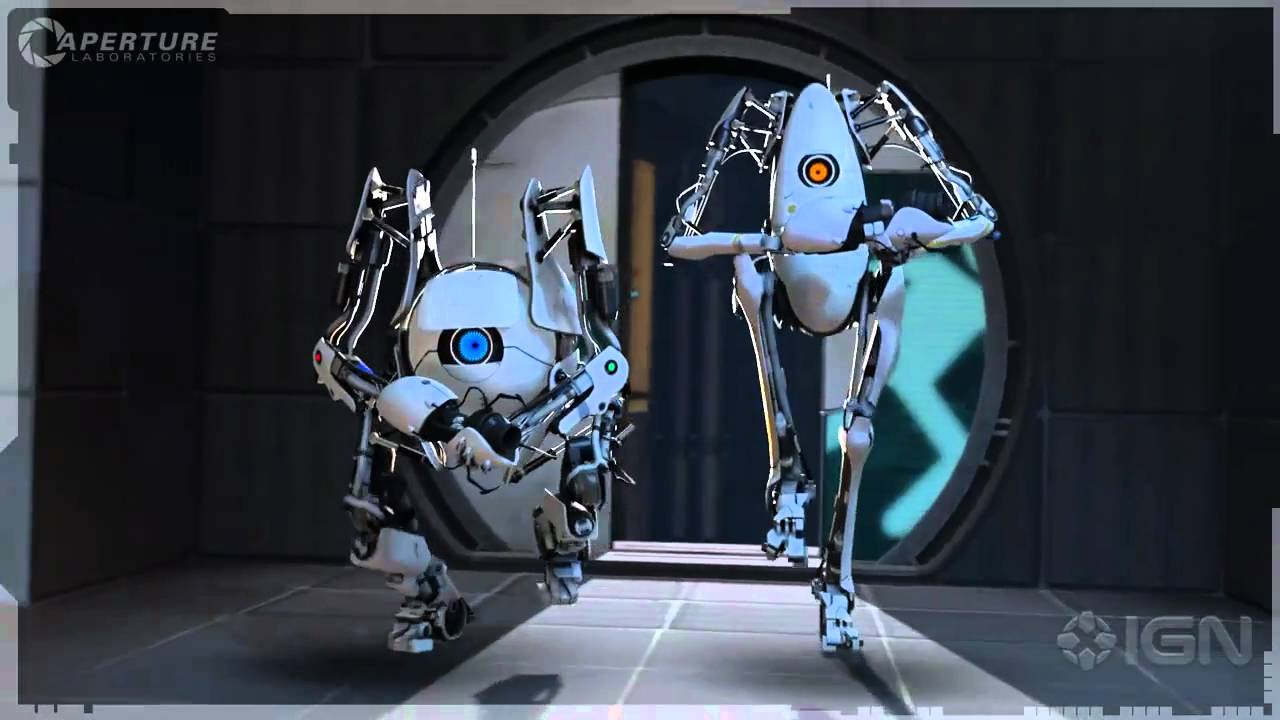
\includegraphics[width=0.6\textwidth]{img/coop.jpg}

vs
\vspace{0.25cm}

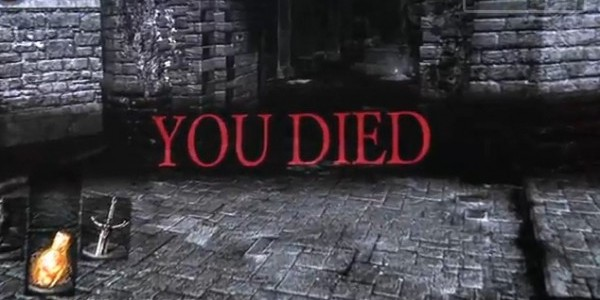
\includegraphics[width=0.6\textwidth]{img/coop_youdied.jpg}
\end{frame}

\section{Eclipse}
\begin{frame}
\begin{enumerate}
\item Java JDK 8u102: \texttt{http://www.oracle.com/technetwork/ java/javase/downloads/}
\item Eclipse: \texttt{https://www.eclipse.org/downloads/}
\item Settings anpassen
\item Tutorial starten
\end{enumerate}

\end{frame}

\begin{frame}{Alternativen}
\begin{description}[align=left]
\item[Java IDEs:] NetBeans
\item[Allgemeine IDEs:] Geany, QtCreator, Visual Studio 2015
\item[Editoren:] VSCode, Atom, Sublime Text, Lightroom, Notepad++, \dots
\item[Harte Editoren:] Emacs oder Vim
\item[Hardmode:] Notepad
\end{description}
\vfill

\hfill
\includegraphics[width=0.2\textwidth]{img/irrelephant.jpg}
\end{frame}

\section{Erstes Programm}
\begin{frame}[fragile]{Hello World}
\begin{lstlisting}
public class HelloWorld 
{ 
  public static void main (String[] args)
  {
    System.out.println("Hello World!");
  }
}
\end{lstlisting}
\end{frame}

\begin{frame}[fragile]{Anatomie Basics}
\begin{lstlisting}
public class [Klassenname] 
{ 
  // public   = Überall sichtbar
  // static   = benötigt kein Objekt
  // main     = Programm startet hier 
  // String[] = mehrere Stücke Text
  // args     = Variable mit Argumenten
  public static void main (String[] args) 
  {
    // Hier alle eure Befehle
  }
}
\end{lstlisting}
\end{frame}

\begin{frame}[fragile]{Ausgabe}
\begin{lstlisting}
public class HelloWorld 
{ 
  public static void main (String[] args)
  {
    System.out.println("Text!");
    System.out.println(42);
    WierdObject wtf;
    System.out.println(wtf.toString());
  }
}
\end{lstlisting}
\end{frame}

\begin{frame}[fragile]{Eclipse Tipps}
\begin{itemize}
\item \texttt{main} + \texttt{Space} = Main-Methode
\item \texttt{Syso} + \texttt{Space} = \texttt{System.out.println}
\item \texttt{Ctrl+Shift+F} = Offene Datei formatieren
\item \texttt{Ctrl-1} = Quick fix
\item Kontextmenü "Source" und "Refactor" sehr praktisch
\end{itemize}
\end{frame}

\begin{frame}[fragile]{Fehlersuche}
  \begin{lstlisting}
System.out.println("Hello World")


Exception in thread "main" java.lang.Error: Unresolved compilation problem: 
    Syntax error, insert ";" to complete Statement

    at Exampleclass.main(Exampleclass.java:10)
  \end{lstlisting}
\end{frame}

\begin{frame}[fragile]{Fehlersuche}
  \begin{lstlisting}
public static int value()
{
    return 5;
	
    
Exception in thread "main" java.lang.Error: Unresolved compilation problem: 
    Syntax error, insert "}" to complete MethodBody

    at Exampleclass.main(Exampleclass.java:11)
  \end{lstlisting}
\end{frame}

\begin{frame}[fragile]{Fehlersuche}
  \begin{lstlisting}
int x = 1/0;


Exception in thread "main" java.lang.ArithmeticException: / by zero
    at Exampleclass.main(Exampleclass.java:13)
  \end{lstlisting}
\end{frame}

\begin{frame}[fragile]{Fehlersuche}
  \begin{lstlisting}
for (float i = 0; i < 1.0; i += 0.1)
{
    System.out.println(i);
}

0.0
0.1
0.2
0.3
0.4
0.5
0.6
0.70000005 // wat?
0.8000001
0.9000001
  \end{lstlisting}
\end{frame}

\begin{frame}{Fehlersuche}
  \centering
  
\includegraphics[width=0.8\textwidth]{img/justgoogle.jpg}
\end{frame}

\begin{frame}{Fehlersuche}
  \begin{enumerate}
  \item Fehlermeldung lesen
  \item Alle eigenen Namen und Pfade löschen
  \item "Java + [deine Fehlermeldung] googeln
  \item Bei Stackoverflow \& Co auch weiter runterscrollen
  \item Kommilitonen und/oder Tutor fragen
  \end{enumerate}
\end{frame}

\end{document}
